\section{Physical view}

\begin{figure}[h]
  \centering
  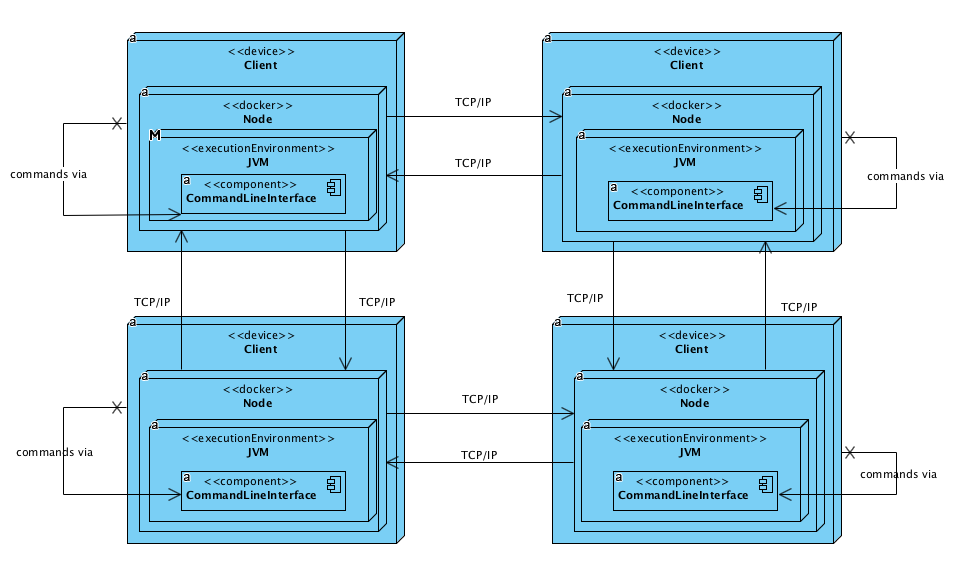
\includegraphics[width=1\textwidth]{deployment}
  \caption{Deployment Diagram}
  \label{model:deployment}
\end{figure}

In het Deployment Diagram is te zien dat er gebruik gemaakt wordt van Docker om de Blockchain client te draaien. Een vereiste hiervan is dat de Docker container beschikking heeft over de Java Virtual Machine. Communicatie tussen Blockchain clients gebeurt over TCP/IP waardoor een internetconnectie een vereiste is.

\subsection{Software Dependencies}

Om de applicatie te laten werken in de Docker container zijn er een aantal software modules nodig:

\begin{tabular}{|p{3cm}|p{10cm}|}
  \hline
  \textbf{Module} & \textbf{Beschrijving} \\
  \hline
  Maven & Wordt gebruikt om alle dependencies op te halen, en tevens het build proces uit te voeren. \\
  \hline
  RocksDB & Verzorgd de opslag binnen de applicatie. \\
  \hline
\end{tabular}